\section{EMPIRICAL EVALUATION}
\label{sec:results}
In this section, we evaluate the performance of our system using a real-world event streams provided by the datAcron project in the context of maritime monitoring. The used event streams describe critical points (i.e., synopses) of moving vessels trajectories, which are derived from raw AIS messages as was  described in \cite{synopses1}. In particular, for our evaluation experiments we used a data set of synopses contains $4,684,444$ critical points of $5055$ vessels sailing in the Atlantic Ocean during the period from 1 October 2015 to 31 March 2016. We used it to generate a simulated stream of event tuples  \textit{(id,timestamp, longitude, latitude, annotation, speed, heading)}, which are processed by the system to attach another field \textit{type} that represents the event value,  where $type$ $\in \Sigma$,  and $ \Sigma= \Sigma_1=$$\{$\textit{VerySlow ,Slow, Moving, Sailing, Stopping} $\}$ , which is based on ranging the speed values. Or $\Sigma=\Sigma_2=$ $\{$  \textit{stopStart,stopEnd, changeInSpeedStart, changeInSpeedEnd, slowMotionStart, slowMotionEnd, gapStart, gapEnd,   changeInHeading} $\}$, which is derived based on the values of the $annotation$ attribute that encodes the extracted trajectory movement events \cite{synopses1}. In our experiments, we monitor a pattern $\mathcal{P}_1=Sailing$ with $m=2$ over $\Sigma_1$ that detects when the vessel under way (sailing). In addition, we test a second pattern  $\mathcal{P}_2=$\textit{changeInHeading; gapStart; gapEnd; changeInHeading} with $m=1$ over $\Sigma_2$.


\subsubsection*{Experimental setup} We ran our experiments on single-node standalone Flink cluster deployed on a server (Ubuntu 17.04) with Intel(R) Core(TM) i7-7700 CPU @ 3.60GHz X 8 processors and 32GB RAM. We used Apache Flink v1.3.2 and Apache Kafka v0.10.2.1 for our tests.


\subsubsection*{Evaluation criteria} Our goal is to evaluate our distributed pattern prediction system, which enables the synchronization of prediction models(i.e., PMC models) on the distributed predictor nodes. Our proposed system can operate with three different flavors of synchronization schemes: \begin{enumerate*}[label=(\roman*)] 
	\item static based on synchronizing the prediction models periodically every $b$ of input events, 
\item continuous synchronization for each incoming event (hypothetical), 
\item dynamic synchronization based on making the predictors communicate their prediction models periodically only when the divergence of the models form a reference model exceeds a variance threshold $\Delta$ (recommended).
 	   
\end{enumerate*}
We compare our proposed system against the isolated prediction approach (i.e., without exchanging information), we compare the predictive performance in terms of :
\begin{enumerate*}[label=(\roman*)]
	
\item  $\mathit{precision = \frac{\#\ of\ correct\ predictions}{\#\ of\ total\ predictions}}$ is the percent of the produced predictions are correct (i.e., a full match occurred within the prediction interval).   

\item $\mathit{recall}$ is the fraction of the full matches of the pattern are successfully predicted by the system at least once. 

\end{enumerate*} 
\par Moreover, we study the communication cost by measuring the $\mathit{cumulative\ communication}$ that captures the number of messages are required to perform the distributed online learning to synchronize the prediction models. In next, we present the experimental results for the for the pattern  $\mathcal{P}_1=Sailing$ with $m=2$, batch size $b=100$, variance threshold $\Delta=2$, and PMC prediction threshold $\theta_{fc}=80\%$.

\begin{figure}[]
	
	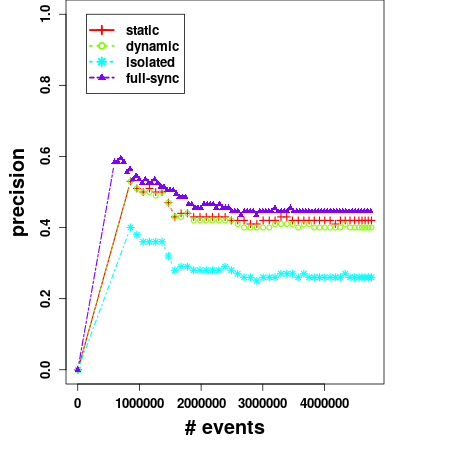
\includegraphics[width=.5\textwidth]{figures/precision.png}
	
	\caption{Precision scores with respect to the total number of input events over time for the pattern $\mathcal{P}_1$.}
	\label{fig:precsions}
\end{figure}

\subsubsection*{Experimental results} Figure ~\ref{fig:precsions} depicts the average precision scores of predictions models (one prediction model per vessel) of all approaches, namely, isolated without synchronization, continuous, static, and our recommended approach based on the dynamic synchronization scheme. It can be clearly seen that all methods of distributed learning outperform the isolated prediction models. The most complex method, continuous synchronization, has the higher precision rates, while the static and dynamic synchronization schemes have a similar precision scores. 
\par In addition, Figure ~\ref{fig:comm} provides the accumulated communication required for the three approaches based on the distributed online learning, while, the isolated approach does not require any communication between the models. As expected, a larger amount of communication is required for the continuous synchronization comparing to the static and dynamic approaches, and it can bee seen that we can reduce the communication overhead by applying the dynamic synchronization protocol (a reduction by a factor of 100) comparing to the static synchronization scheme, even with a small variance threshold $\Delta=2$. Furthermore, the dynamic method is still preserving a similar predictive performance of the static one as shown in Figure ~\ref{fig:precsions}.    





\begin{figure}[]
	
	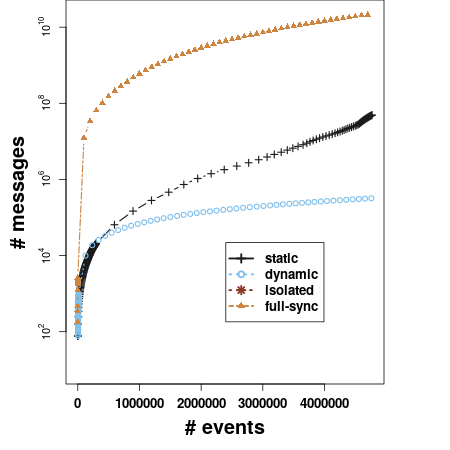
\includegraphics[width=.5\textwidth]{figures/communication.png}
	
	\caption{Commutative communication with respect to the total number of input events over time for the pattern $\mathcal{P}_1$.}
	\label{fig:comm}
\end{figure}


\par In Table ~\ref{tab:recall}, we present the statistics of recall results for the different approaches. It can be seen 

\begin{table}[]
	\caption{Recall results.}
	\label{tab:recall}
	\begin{tabular}{lcc}
		\toprule
		Approach &Mean recall for $\mathcal{P}_1$ &Mean recall for $\mathcal{P}_2$\\
		\midrule
		isolated & 0.1707  & 0.860 \\
		static & 0.1754  &  0.970 \\
		dynamic & 0.174  & 0.962 \\
		full-sync & 0.1817  & 0.972 \\
		\bottomrule
	\end{tabular}
\end{table}


 
